\chapter{初边值问题}

这里考虑一维问题的边界处理,边界条件分为:
\begin{enumerate}
    \item Dirichlet 边界条件:本质边界条件
    \item Neumann、Robin 边界条件:自然边界条件
\end{enumerate}

\section{一维扩散方程的边界处理}

对于 $u_t =  u_{xx}$,以左边界 $x=0$ 的混合边界条件为例
\[
    - a u_x(0,t) + \sigma u(0,t) = \varphi_0(t),\quad (\sigma \ge 0)
\]
可以直接基于微分形式做近似,有如下的边界处理方法:
\begin{enumerate}
    \item 单侧差商离散
          \[
              -a \frac{v_1^n - v_0^n}{\Delta x} + \sigma v_0^n = \varphi_0(t^n)
          \]
    \item 双侧离散方法:
          \begin{enumerate}
              \item 虚拟点方法:$x_{-1} = - \Delta x$,$x_0 = 0$(如图~\ref{fig:discrete-grid}),有两种做法
                    \begin{align*}
                        \text{(1)} \quad & -a \frac{v_1^n - v_{-1}^n}{2\Delta x} + \sigma v_0^n = \varphi_0(t^n)
                        \\
                        \text{(2)} \quad & -a \frac{v_1^n - v_{-1}^n}{2\Delta x} + \sigma \frac{v_{-1}^n + v_1^n }2  = \varphi_0(t^n)
                    \end{align*}
              \item 半网格法:$x_0 = -{\Delta x}/2$,$x_1 = {\Delta x}/2$(如图~\ref{fig:discrete-grid})
                    \[
                        -a \frac{v_1^n - v_{0}^n}{\Delta x} + \sigma \frac{v_0^n + v_1^n}2 = \varphi_0(t^n)
                    \]
          \end{enumerate}
\end{enumerate}
也可以基于积分形式进行近似,例如取 $[x_0,x_{1/2}] \times [t^n,t^{n+1}]$ 积分可得
\begin{gather*}
    \frac{\Delta x}2 (v_0^{n+1} - v_0^n)
    = \Delta t a \frac{v_1^n - v_0^n}{\Delta x} + \Delta t (\varphi_0(t^n) - \sigma u_0^n)
    \\
    \Rightarrow \quad  v_0^{n+1} = \left(1 - \frac{2 a \Delta t}{\Delta x^2} - \frac{2\sigma \Delta t}{\Delta x}\right) v_0^n
    + \frac{2 a \Delta t}{\Delta x^2} v_1^n + \frac{2\Delta t}{\Delta x} \varphi_0(t^n)
\end{gather*}


\begin{figure}[htbp]
    \centering
    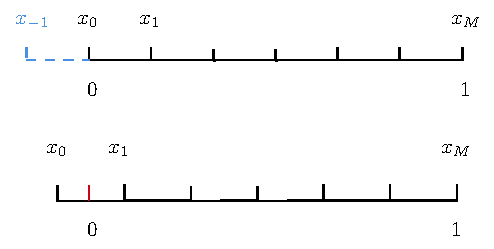
\includegraphics[width=.5\textwidth]{tikz/discrete-grid.pdf}
    \caption{整网格(以及左侧虚拟点)和(左侧)半网格示意图} \label{fig:discrete-grid}
\end{figure}

\section{一维对流方程的边界处理}

对流方程的边界条件设置需要根据风向确定,例如对于入流边界 $x=1$ 和出流边界 $x=0$,
只有入流边界需要提供边界条件 $u(1,t) = \varphi(t)$,对于出流边界不应该提供边界条件,差分格式在处理出流边界时通常有如下办法:
\begin{enumerate}
    \item 对于单边迎风格式,此时无需特殊的边界处理;
    \item 对于 Lax-Wendroff 格式,Lax–Friedrichs 格式等双边离散的格式,需要设计人工出流边界,即更新 $v_0^{n+1}$ 的公式:包括直接利用内部点外插,以及利用特征线求解等。
\end{enumerate}


\section{初边值问题的性质分析}

初值问题与初边值问题的差分格式在分析时的最大区别:
\begin{itemize}
    \item 初值问题:$\Delta x$ 减小时,考虑的空间序列仍是同一个序列空间(无限维空间);
    \item 初边值问题:$\Delta x$ 减小时,考虑的空间序列会发生变化(空间维度逐渐提升的有限维空间)。没有一个合适的空间可以定义差分格式的收敛性,必须考虑一个变化的空间序列以及相应的模序列。
\end{itemize}


考虑有界区域 $[0,1]$,默认考虑均匀剖分并对网格逐渐加密:设第 $k$ 个网格含两侧边界的格点数为 $M_k+1$,
网格尺度 $\Delta x^{(k)} = \frac{1}{M_k}$,满足 $\Delta x^{(k)} \to 0\,(k \to \infty)$。
第 $k$ 个网格的离散点序列为
\[
    0 = x_0^{(k)} < x_1^{(k)} < \cdots < x_{M_k}^{(k)} = 1, \quad x_j^{(k)} = j \Delta x^{(k)}.
\]
对应的数值解和精确解记作
\[
    V^{n,(k)} = \{v_0^{n,(k)},v_1^{n,(k)},\cdots,v_{M_k}^{n,(k)}\}, \quad
    U^{n,(k)} = \{u_0^{n,(k)},u_1^{n,(k)},\cdots,u_{M_k}^{n,(k)}\}
\]
对应的有限维空间 $X^{(k)}$ 具有范数 $\|\cdot\|_k$。

\subsection{相容性}

\begin{definition}[局部截断误差]
    对于偏微分方程 $\mathcal{L} u = g$ 以及对应的差分格式 $L v_j^n = g_j^n$,
    定义在 $(x_j,t^n)$ 处的局部截断误差为
    \[
        \tau_j^n = L u_j^n - g_j^n - (\mathcal{L}u(x_j,t^n) - g(x_j,t^n)) = L u_j^n - g_j^n
    \]
    其中 $u(x,t)$ 是满足偏微分方程的充分光滑函数。在内部和边界计算得到的局部截断误差可能不一样。
\end{definition}

\begin{definition}[逐点相容性]
    称偏微分方程 $\mathcal{L} u = g$ 对应的差分格式 $L v_j^n = g_j^n$ 是(无条件)逐点相容的:如果局部截断误差 $\tau_j^n$ 在
    $\Delta x^{(k)},\Delta t^{(k)}\to 0$ 时满足
    \[
        \tau_j^n \to 0.
    \]
    进一步,称这个格式的局部截断误差阶是 $(p,q)$ :如果存在不可改善的正数 $p,q$,使得下式成立
    \[
        \tau_j^n = \mathcal{O}((\Delta x^{(k)})^p + (\Delta t^{(k)})^q)
    \]
    由于通常对内部和边界采用了不同的近似处理,在内部和边界计算得到的局部截断误差阶可能不一样,差分格式的局部截断误差阶取两者中的最小值。
\end{definition}



\begin{definition}[模相容性]\label{def:ib-norm-consistency}
    对于初边值问题的双层格式
    \[
        V^{n+1,(k)} = Q \, V^{n,(k)} + \Delta t^{(k)}\, G^{n,(k)}
    \]
    将满足偏微分方程的充分光滑函数 $U$ 代入会产生余项 $\Delta t^{(k)}\, T^{n,(k)}$
    \[
        U^{n+1,(k)} = Q \, U^{n,(k)} + \Delta t^{(k)}\, G^{n,(k)} + \Delta t^{(k)}\, T^{n,(k)}
    \]
    称差分格式是(无条件)关于 $\|\cdot\|_k$ 模相容的:
    如果随着 $k \to \infty$,$\Delta t^{(k)} \to 0$,$n \Delta t^{(k)} \to t^*$,有
    \[
        \|T^{n,(k)}\|_{k} \to 0
    \]
    进一步,称这个格式的 $\|\cdot\|_k$ 模相容阶是 $(p,q)$:如果存在不可改善的正数 $p,q$,使得下式成立
    \[
        \|T^{n,(k)}\|_{k} = \mathcal{O}((\Delta x^{(k)})^p + (\Delta t^{(k)})^q)
    \]
\end{definition}

\begin{remark}
    对于初边值问题,整理为向量形式的差分格式是包括内部离散和边界离散的,尤其注意的是,对于边界附近的点值,实际的计算格式是由内部离散和边界离散耦合得到的。
\end{remark}

\begin{remark}
    对于隐格式,通常可以整理为如下形式
    \[
        P V^{n+1,(k)} = Q \, V^{n,(k)} + \Delta t^{(k)}\, G^{n,(k)}
    \]
    此时不需要计算 $P^{-1}$ 来整理为定义~\ref{def:ib-norm-consistency} 中的形式,直接将精确解代入格式两侧
    \[
        P U^{n+1,(k)} = Q \, U^{n,(k)} + \Delta t^{(k)}\, G^{n,(k)} + \Delta t^{(k)}\, T^{n,(k)}
    \]
    模相容性仍然通过 $T^{n,(k)}$ 来体现。
\end{remark}

\begin{remark}
    这里采用了教材 J.W.Thomas《Numerical Partial Differential Equations: Finite Difference Methods》2.3.2 节中的观点:
    逐点相容性只考虑内部差分格式对于偏微分方程的近似,或只考虑边界离散处理对边界条件的近似效果,并不考虑两者的耦合;
    模相容性则是考虑两者在边界附近的耦合得到的实际格式。
    但是这种观点与张强《偏微分方程的有限差分方法》3.4 节并不一致,后者所讨论的局部截断误差是针对两者耦合之后的实际格式进行的分析。
    不过两本教材的相关例子都说明了不合适的边界离散会导致整体出现掉阶现象。
\end{remark}

\subsection{稳定性}

\begin{definition}[模稳定性]
    对于初边值问题的双层格式
    \[
        V^{n+1} = Q \, V^{n}
    \]
    称差分格式是关于 $\|\cdot\|_k$ 模稳定的:
    如果存在常数 $K,\beta > 0$,以及正的 $\Delta x_0,\Delta t_0$,
    使得对于任意 $0 < \Delta x^{(k)} \le \Delta x_0$、$0 < \Delta t^{(k)} \le \Delta t_0$,
    以及 $0 \le t = (n+1)\Delta t^{(k)}$,有
    \[
        \|V^{n+1,(k)}\|_{k} \le K e^{\beta t} \| V^{0,(k)}\|_k
    \]
\end{definition}

根据定义很容易得到模稳定性的充要条件:
\begin{theorem}
    对于初边值问题的双层差分格式
    \[
        V^{n+1} = Q \, V^{n}
    \]
    差分格式是关于 $\|\cdot\|_k$ 模稳定的充要条件是:
    存在常数 $K,\beta > 0$,以及正的 $\Delta x_0,\Delta t_0$,
    使得对于任意 $0 < \Delta x^{(k)} \le \Delta x_0$、$0 < \Delta t^{(k)} \le \Delta t_0$,
    以及 $0 \le t = (n+1)\Delta t^{(k)}$,有
    \[
        \|Q^{n+1}\|_{k} \le K e^{\beta t}
    \]
\end{theorem}

如果特别取 $\|\cdot\|_k$ 为具体的模,可以得到一些与矩阵 $Q$ 相关的稳定性条件。

\begin{theorem}
    对于初边值问题的双层差分格式
    \[
        V^{n+1} = Q \, V^{n}
    \]
    关于 $\|\cdot\|_{2,k}$ 模稳定的必要条件是:
    存在常数 $C \ge 0$,使得
    \[
        \sigma(Q) = \max_i|\lambda_i(Q)| \le 1 + C\,\Delta t
    \]
\end{theorem}

\begin{theorem}
    对于初边值问题的双层差分格式
    \[
        V^{n+1} = Q \, V^{n}
    \]
    关于最大模 $\|\cdot\|_{\infty,k}$ 稳定的一个充分条件是 $\|Q\|_{\infty,k} \le 1$。
\end{theorem}

\subsection{收敛性}


\begin{definition}[模收敛性]
    对于初边值问题的双层差分格式
    \[
        V^{n+1,(k)} = Q \, V^{n,(k)} + \Delta t^{(k)}\, G^{n,(k)}
    \]
    称这个格式是(无条件)关于 $\|\cdot\|_k$ 模收敛的:如果随着 $k \to \infty$,$\Delta t^{(k)} \to 0$,$(n+1) \Delta t^{(k)} \to t^*$,有
    \[
        \|U^{n+1,(k)} - V^{n+1,(k)}\|_{k} \to 0
    \]
    其中 $U$ 是满足偏微分方程的充分光滑函数。
    进一步,称这个格式关于 $\|\cdot\|_k$ 模的收敛阶是 $(p,q)$:如果存在不可改善的正数 $p,q$,使得下式成立
    \[
        \|U^{n+1,(k)} - V^{n+1,(k)}\|_{k} = \mathcal{O}((\Delta x^{(k)})^p + (\Delta t^{(k)})^q)
    \]
\end{definition}


\subsection{Lax定理}


\begin{theorem}[Lax定理]
    对于一个适定的线性偏微分方程初边值问题的双层差分格式
    \[
        V^{n+1,(k)} = Q \, V^{n,(k)} + \Delta t\, G^{n,(k)}
    \]
    若其关于 $\|\cdot\|_k$ 模的相容阶是 $(p,q)$,并且它关于 $\|\cdot\|_k$ 模稳定,那么该格式关于 $\|\cdot\|_k$ 模的收敛阶是 $(p,q)$。
\end{theorem}

\subsection{一些例子}

主要关注一维常系数扩散方程的初边值问题分析。

\subsubsection{Dirichlet边界}

考虑如下扩散方程初边值问题($b > 0$),左右均为Dirichlet边界
\[
    \left\{
    \begin{aligned}
         & u_t = b u_{xx},      &  & x \in (0,1),\, t > 0, \\
         & u(x,0) = u_0(x),     &  & x \in [0,1],          \\
         & u(0,t) = u(1,t) = 0, &  & t \ge 0.
    \end{aligned}
    \right.
\]
在边界直接赋值,得到差分格式(记 $\mu = \frac{ b \Delta t}{\Delta x^2}$)
\begin{equation}
    \left\{
    \begin{aligned}
         & v_j^{n+1} = v_j^n + \mu \delta_x^2 v_j^n, &  & j=1,\dots,M_k-1,\, n=0,1,\dots, \\
         & v_j^0 = u_0(x_j),                         &  & j=0,\dots,M_k,                  \\
         & v_0^{n+1} = v_{M_k}^{n+1} = 0,            &  & n=0,1,\dots.
    \end{aligned}
    \right. \label{eq:ib-1}
\end{equation}


\begin{example}
    当 $0 < \mu \le \frac12$ 时,差分格式~\eqref{eq:ib-1} 关于最大模 $\|\cdot\|_{\infty}$ 稳定 \& 收敛。
\end{example}

\begin{proof}
    直接放缩可以证明最大模稳定性
    \begin{align*}
        v_{j}^{n+1} ={}     &
        v_j^{n} + \mu (v_{j+1}^{n}-2v_j^{n}+v_{j-1}^{n})                        \\
        ={}                 & \mu v_{j+1}^{n} + (1-2\mu)v_j^{n}+\mu v_{j-1}^{n} \\
        |v_{j}^{n+1}| \le{} &
        \mu |v_{j+1}^{n}| + (1-2\mu)|v_j^{n}|+\mu |v_{j-1}^{n}| \le{}  \|V^{n}\|_{\infty}
    \end{align*}
    因此 $\|V^{n+1}\|_{\infty} \le{} \|V^{n}\|_{\infty}$。

    对于数值解 $v_{j}^{n+1}$ 和精确解 $u_{j}^{n+1}$,满足
    \begin{align*}
        v_{j}^{n+1} & = v_j^{n} + \mu \delta_x^2 v_j^{n},                       \\
        u_{j}^{n+1} & = u_j^{n} + \mu \delta_x^2 u_j^{n} + \Delta t \tau_j^{n},
    \end{align*}
    其中局部截断误差为 $\tau_j^{n} = \mathcal{O}(\Delta x^2 + \Delta t)$。
    将两式作差,定义 $z_{j}^{n+1}=u_{j}^{n+1}-v_{j}^{n+1}$
    \begin{align*}
        z_{j}^{n+1} ={}     &
        z_j^{n} + \mu (z_{j+1}^{n}-2z_j^{n}+z_{j-1}^{n}) + \Delta t \tau_j^{n}
        \\
        ={}                 & \mu z_{j+1}^{n} + (1-2\mu)z_j^{n}+\mu z_{j-1}^{n}+ \Delta t \tau_j^{n}
        \\
        |z_{j}^{n+1}| \le{} &
        \mu |z_{j+1}^{n}| + (1-2\mu)|z_j^{n}| + \mu |z_{j-1}^{n}| + \Delta t A (\Delta x^2 + \Delta t)
        \\
        \le{}               & \|Z^{n}\|_{\infty}+ \Delta t A (\Delta x^2 + \Delta t)
    \end{align*}
    遍历所有的 $j$ 使得左侧取到最大值 $\|Z^{n+1}\|_{\infty}$,可得
    \begin{align*}
        \|Z^{n+1}\|_{\infty} \le{} & \|Z^{n}\|_{\infty}+ \Delta t A (\Delta x^2 + \Delta t)
        \\ \le{} & \cdots \le (n+1)\Delta t A (\Delta x^2 + \Delta t) \\
        ={}                        & t^* A (\Delta x^2 + \Delta t) \to 0.
    \end{align*}
    得证最大模收敛性,最大模收敛阶为 $(2,1)$。
\end{proof}


\subsubsection{Neumann、Robin 边界(整网格)}

考虑如下扩散方程初边值问题($b > 0$),左侧为Robin 边界($\sigma \ge 0$),右侧为Dirichlet边界
\[
    \left\{
    \begin{aligned}
         & u_t = b u_{xx},                 &  & x \in (0,1),\, t > 0, \\
         & u(x,0) = u_0(x),                &  & x \in [0,1],          \\
         & - u_x(0,t) + \sigma u(0,t) = 0, &  & t \ge 0,              \\
         & u(1,t) = 0,                     &  & t \ge 0.
    \end{aligned}
    \right.
\]
左侧边界使用单侧差商离散
\[
    -  \frac{v_1^n - v_0^n}{\Delta x} + \sigma v_0^n = 0, \quad \Rightarrow \quad v_0^n = \frac{1}{1 + \sigma \Delta x} v_1^n
\]
得到差分格式(记 $\mu = \frac{b \Delta t}{\Delta x^2}$)
\begin{equation}
    \left\{
    \begin{aligned}
         & v_j^{n+1} = v_j^n + \mu \delta_x^2 v_j^n,            &  & j=1,\dots,M_k-1,\, n=0,1,\dots, \\
         & v_j^0 = u_0(x_j),                                    &  & j=0,\dots,M_k,                  \\
         & v_0^{n+1} = \frac{1}{1 + \sigma \Delta x} v_1^{n+1}, &  & n=0,1,\dots.                    \\
         & v_{M_k}^{n+1} = 0,                                   &  & n=0,1,\dots.
    \end{aligned}
    \right.    \label{eq:ib-2}
\end{equation}

\begin{example}
    当 $0 < \mu \le \frac12$ 时,差分格式~\eqref{eq:ib-2} 在最大模 \& $L^2$ 模意义下是稳定的。
\end{example}

\begin{proof}
    将格式写作 $V^{n+1} = Q\, V^n$ 的形式(不含 $v_0$ 和 $v_{M}$)
    \[
        \begin{bmatrix}
            v_1^{n+1} \\ v_2^{n+1} \\ \vdots \\ v_{M-2}^{n+1} \\ v_{M-1}^{n+1}
        \end{bmatrix}
        =
        \begin{bmatrix}
            1-2\mu + \frac{\mu}{1+\sigma \Delta x} & \mu    &        &        &        \\
            \mu                                    & 1-2\mu & \mu    &        &        \\
                                                   & \ddots & \ddots & \ddots &        \\
                                                   &        & \mu    & 1-2\mu & \mu    \\
                                                   &        &        & \mu    & 1-2\mu \\
        \end{bmatrix}
        \begin{bmatrix}
            v_1^{n} \\ v_2^{n} \\ \vdots \\ v_{M-2}^{n} \\ v_{M-1}^{n}
        \end{bmatrix}
    \]
    稳定性只需要证明无穷范数 $\|Q\|_{\infty} \le 1$
    和谱半径 $\sigma(Q) \le 1$,对于矩阵 $Q$,这两个结论显然成立。
\end{proof}

\begin{example}
    差分格式~\eqref{eq:ib-2} 是逐点相容的。
\end{example}

\begin{proof}
    对于内部离散,将精确解 $u$ 代入可得
    \[
        \tau_j^n = \frac{u_{j}^{n+1}-u_j^n}{\Delta t} - \frac{u_{j+1}^{n}-2u_{j}^{n}+u_{j-1}^{n}}{\Delta x^2}
        = \mathcal{O}(\Delta x^2 + \Delta t)
    \]
    对于边界离散,将精确解 $u$ 代入可得
    \[
        \tau_0^n = - \frac{u_1^n - u_0^n}{\Delta x} + \sigma u_0^n = \mathcal{O}(\Delta x)
    \]
    因此格式是逐点相容的,局部截断误差阶是 $(1,1)$。
\end{proof}

\begin{example}
    差分格式~\eqref{eq:ib-2} 是最大模不相容的。
\end{example}

\begin{proof}
    将精确解 $u$ 代入格式~\eqref{eq:ib-2} 的矩阵形式,产生余项 $\Delta t\, T^n$
    \[
        \begin{bmatrix}
            u_1^{n+1} \\ u_2^{n+1} \\ \vdots \\ u_{M-2}^{n+1} \\ u_{M-1}^{n+1}
        \end{bmatrix}
        =
        \begin{bmatrix}
            1-2\mu + \frac{\mu}{1+\sigma \Delta x} & \mu    &        &        &        \\
            \mu                                    & 1-2\mu & \mu    &        &        \\
                                                   & \ddots & \ddots & \ddots &        \\
                                                   &        & \mu    & 1-2\mu & \mu    \\
                                                   &        &        & \mu    & 1-2\mu \\
        \end{bmatrix}
        \begin{bmatrix}
            u_1^{n} \\ u_2^{n} \\ \vdots \\ u_{M-2}^{n} \\ u_{M-1}^{n}
        \end{bmatrix}
        +
        \Delta t
        \begin{bmatrix}
            T_1^{n} \\ T_2^{n} \\ \vdots \\ T_{M-2}^{n} \\ T_{M-1}^{n}
        \end{bmatrix}
    \]
    易知 $T_j^{n} = \mathcal{O}( \Delta x^2 + \Delta t)$,$j=2,\dots,M-1$,
    只需要关注 $T_1^{n}$
    \begin{align*}
        \Delta t\, T_1^{n} ={} & u_1^{n+1} - \left(1-2\mu + \frac{\mu}{1+\sigma \Delta x}\right) u_1^n - \mu u_2^n \\
        ={}                    & \mu \left(u_0^n - \frac{1}{1+\sigma \Delta x} u_1^n\right)
        + \left[
        u_1^{n+1} - u_1^n - \mu(u_0^n - 2 u_1^n + u_2^n)
        \right]                                                                                                    \\
        ={}                    & \mu \left(u_0^n - \frac{1}{1+\sigma \Delta x} u_1^n\right)
        + \mathcal{O}(\Delta t \Delta x^2 + \Delta t^2)
    \end{align*}
    由边界条件可得
    \begin{gather*}
        -  \frac{u_1^n - u_0^n}{\Delta x} + \sigma u_0^n = -\frac{\Delta x}2 (u_{xx})_1^n + \mathcal{O}(\Delta x^2),\\
        u_0^n - \frac{u_1^n}{1+\sigma \Delta x} = -\frac{\Delta x^2}2 (u_{xx})_1^n + \mathcal{O}(\Delta x^3).
    \end{gather*}
    代入可得
    \[
        \Delta t\, T_1^{n} ={} -\frac{b \Delta t}2 (u_{xx})_1^n + \mathcal{O}(\Delta t^2 \Delta x)+ \mathcal{O}(\Delta t \Delta x^2 + \Delta t^2)
    \]
    因此 $T_1^n = \mathcal{O}(1)$,这直接导致 $\|T^n\|_{\infty} = \mathcal{O}(1)$,因此格式按最大模不相容。
\end{proof}

左侧边界引入虚拟点 $x_{-1}$ 进行双侧离散,得到
\[
    - \frac{v_{1}^{n}-v_{-1}^{n}}{2\Delta x} + \sigma v_0^n = 0, \quad \Rightarrow \quad v_{-1}^{n} = v_0^{n} - 2\sigma \Delta x v_0^n.
\]
得到差分格式(记 $\mu = \frac{b \Delta t}{\Delta x^2}$)
\begin{equation}
    \left\{
    \begin{aligned}
         & v_j^{n+1} = v_j^n + \mu \delta_x^2 v_j^n,                    &  & j=1,\dots,M_k-1,\, n=0,1,\dots, \\
         & v_j^0 = u_0(x_j),                                            &  & j=0,\dots,M_k,                  \\
         & v_0^{n+1} = v_0^n + 2\mu (v_1^n-(1+ \sigma \Delta x) v_0^n), &  & n=0,1,\dots.                    \\
         & v_{M_k}^{n+1} = 0,                                           &  & n=0,1,\dots.
    \end{aligned}
    \right.
    \label{eq:ib-3a}
\end{equation}
还可以将 $v_0^n$ 用空间平均替代,使用如下方式离散
\[
    - \frac{v_{1}^{n}-v_{-1}^{n}}{2\Delta x} + \sigma \frac{v_{-1}^n + v_1^n}2 = 0, \quad \Rightarrow \quad v_{-1}^{n} = \frac{1-\sigma \Delta x}{1+\sigma \Delta x} v_1^n.
\]
得到差分格式(记 $\mu = \frac{b \Delta t}{\Delta x^2}$)
\begin{equation}
    \left\{
    \begin{aligned}
         & v_j^{n+1} = v_j^n + \mu \delta_x^2 v_j^n,                                      &  & j=1,\dots,M_k-1,\, n=0,1,\dots, \\
         & v_j^0 = u_0(x_j),                                                              &  & j=0,\dots,M_k,                  \\
         & v_0^{n+1} = v_0^n + 2\mu \left(\frac{1}{1+\sigma \Delta x}v_1^n- v_0^n\right), &  & n=0,1,\dots.                    \\
         & v_{M_k}^{n+1} = 0,                                                             &  & n=0,1,\dots.
    \end{aligned}
    \right.    \label{eq:ib-3b}
\end{equation}


\begin{example}
    分析差分格式~\eqref{eq:ib-3a} 和~\eqref{eq:ib-3b} 的最大模稳定性。
\end{example}

\begin{proof}
    将格式~\eqref{eq:ib-3a} 和~\eqref{eq:ib-3b} 写作 $V^{n+1} = Q\, V^n$ 的形式(不含 $v_{M}$)
    \[
        \begin{bmatrix}
            v_0^{n+1} \\ v_1^{n+1} \\ \vdots \\ v_{M-2}^{n+1} \\ v_{M-1}^{n+1}
        \end{bmatrix}
        =
        \begin{bmatrix}
            1-2\mu(1+\sigma \Delta x) & 2\mu   &        &        &        \\
            \mu                       & 1-2\mu & \mu    &        &        \\
                                      & \ddots & \ddots & \ddots &        \\
                                      &        & \mu    & 1-2\mu & \mu    \\
                                      &        &        & \mu    & 1-2\mu \\
        \end{bmatrix}
        \begin{bmatrix}
            v_0^{n} \\ v_1^{n} \\ \vdots \\ v_{M-2}^{n} \\ v_{M-1}^{n}
        \end{bmatrix}
    \]
    \[
        \begin{bmatrix}
            v_0^{n+1} \\ v_1^{n+1} \\ \vdots \\ v_{M-2}^{n+1} \\ v_{M-1}^{n+1}
        \end{bmatrix}
        =
        \begin{bmatrix}
            1-2\mu & \frac{2\mu}{1+\sigma \Delta x} &        &        &        \\
            \mu    & 1-2\mu                         & \mu    &        &        \\
                   & \ddots                         & \ddots & \ddots &        \\
                   &                                & \mu    & 1-2\mu & \mu    \\
                   &                                &        & \mu    & 1-2\mu \\
        \end{bmatrix}
        \begin{bmatrix}
            v_0^{n} \\ v_1^{n} \\ \vdots \\ v_{M-2}^{n} \\ v_{M-1}^{n}
        \end{bmatrix}
    \]
    最大模稳定性只需要证明无穷范数 $\|Q\|_{\infty} \le 1$,对于格式~\eqref{eq:ib-3a},这要求
    \[
        2 \mu (1 + \sigma \Delta x) \le 1
    \]
    这表明边界处理导致了稳定性条件需要加强:要求 $\mu < \frac12$ 并且 $\Delta x $ 足够小。
    对于格式~\eqref{eq:ib-3b},最大模稳定性的要求则仍然是通常的 $\mu \le \frac12$。
\end{proof}

\begin{remark}
    这个例子与 Lax-Friedrichs 格式都表明:使用平均值替换可能会改善差分格式的稳定性。
\end{remark}


\begin{example}
    差分格式~\eqref{eq:ib-3a} 和~\eqref{eq:ib-3b} 都是最大模相容的。
\end{example}

\begin{proof}
    只验证格式~\eqref{eq:ib-3b},格式~\eqref{eq:ib-3a} 的分析完全类似。
    将精确解 $u$ 代入格式~\eqref{eq:ib-3b} 的矩阵形式,产生余项 $\Delta t \,T^n$
    \[
        \begin{bmatrix}
            u_0^{n+1} \\ u_1^{n+1} \\ \vdots \\ u_{M-2}^{n+1} \\ u_{M-1}^{n+1}
        \end{bmatrix}
        =
        \begin{bmatrix}
            1-2\mu & \frac{2\mu}{1+\sigma \Delta x} &        &        &        \\
            \mu    & 1-2\mu                         & \mu    &        &        \\
                   & \ddots                         & \ddots & \ddots &        \\
                   &                                & \mu    & 1-2\mu & \mu    \\
                   &                                &        & \mu    & 1-2\mu \\
        \end{bmatrix}
        \begin{bmatrix}
            u_0^{n} \\ u_1^{n} \\ \vdots \\ u_{M-2}^{n} \\ u_{M-1}^{n}
        \end{bmatrix}
        +
        \Delta t
        \begin{bmatrix}
            T_0^{n} \\ T_1^{n} \\ \vdots \\ T_{M-2}^{n} \\ T_{M-1}^{n}
        \end{bmatrix}
    \]
    易知 $T_j^{n} = \mathcal{O}(\Delta x^2 + \Delta t)$,$j=1,\dots,M-1$,只需要关注 $T_0^{n}$
    \begin{align*}
        \Delta t\, T_0^{n} ={} & u_0^{n+1} - (1-2\mu) u_0^n - \frac{2\mu}{1+\sigma \Delta x} u_1^n            \\
        ={}                    & \mu\left(u_{-1}^n - \frac{1-\sigma \Delta x}{1+\sigma \Delta x} u_1^n\right)
        + \left[
        u_0^{n+1} - u_0^n - \mu(u_{-1}^n - 2 u_0^n + u_1^n)
        \right]                                                                                               \\
        ={}                    & \mu\left(u_{-1}^n - \frac{1-\sigma \Delta x}{1+\sigma \Delta x} u_1^n\right)
        + \mathcal{O}(\Delta t \Delta x^2 + \Delta t^2)
    \end{align*}
    由边界条件可得
    \begin{gather*}
        - \frac{u_{1}^{n}-u_{-1}^{n}}{2\Delta x} + \sigma \frac{u_{-1}^n + u_1^n}2 =
        -\frac{\Delta x^2}6 (u_{xxx})_1^n
        + \frac{\sigma \Delta x^2}2 (u_{xx})_1^n
        + \mathcal{O}(\Delta x^4),\\
        u_{-1}^n - \frac{1-\sigma \Delta x}{1+\sigma \Delta x} u_1^n =
        -\frac{\Delta x^3}3 (u_{xxx})_1^n
        +  \sigma \Delta x^3  (u_{xx})_1^n
        + \mathcal{O}(\Delta x^5)
    \end{gather*}
    代入可得
    \[
        \Delta t\, T_0^{n} ={}  b \Delta t \Delta x \left( -\frac13 (u_{xxx})_1^n +\sigma (u_{xx})_1^n \right)
        + \mathcal{O}(\Delta t\Delta x^3) + \mathcal{O}(\Delta t \Delta x^2 + \Delta t^2)
    \]
    因此 $T_0^n = \mathcal{O}(\Delta x + \Delta t)$,$\|T^n\|_{\infty} = \mathcal{O}(\Delta x + \Delta t)$,格式按最大模相容。
\end{proof}

\begin{remark}
    如果 $\sigma = 0$,即边界条件为 $u_x(0,t) = 0$,此时恰可以由方程 $u_t = b u_{xx}$ 推出在边界处 $u_{xxx}(0,t) = 0$,因此 $(u_{xxx})_1^n = \mathcal{O}(\Delta x)$,
    得到 $T_0^n = \mathcal{O}(\Delta x^2 + \Delta t)$,在边界附近不再掉阶。
    下面讨论的几种格式也有类似的现象,即一般边界条件时的最大模相容性会掉阶,但是特别的边界条件 $u_x = 0$ 恰不会掉阶,在下文中不再赘述。
\end{remark}


\subsubsection{Neumann、Robin 边界(半网格)}

考虑如下扩散方程初边值问题($b > 0$),左侧为Robin 边界($\sigma \ge 0$),右侧为Dirichlet边界
\[
    \left\{
    \begin{aligned}
         & u_t = b u_{xx},                 &  & x \in (0,1),\, t > 0, \\
         & u(x,0) = u_0(x),                &  & x \in [0,1],          \\
         & - u_x(0,t) + \sigma u(0,t) = 0, &  & t \ge 0,              \\
         & u(1,t) = 0,                     &  & t \ge 0.
    \end{aligned}
    \right.
\]
和上一节不同的是,这里对左边界采用半网格离散:$x_{0} = \frac{\Delta x}2$,$x_1 = \frac{\Delta x}2$,对右边界仍然使用整网格 $x_{M_k} = 1$。
对左侧边界采用如下方式离散
\[
    - \frac{v_1^n - v_{0}^n}{\Delta x} + \sigma \frac{v_0^n + v_1^n}2 = 0.\quad\Rightarrow\quad v_0^{n} = \frac{1-\frac{\sigma}2 \Delta x}{1 +\frac{\sigma}2 \Delta x}\, v_1^{n}
\]
得到差分格式(记 $\mu = \frac{b \Delta t}{\Delta x^2}$)
\begin{equation}
    \left\{
    \begin{aligned}
         & v_j^{n+1} = v_j^n + \mu \delta_x^2 v_j^n,                                             &  & j=1,\dots,M_k-1,\, n=0,1,\dots, \\
         & v_j^0 = u_0(x_j),                                                                     &  & j=0,\dots,M_k,                  \\
         & v_0^{n+1} = \frac{1-\frac{\sigma}2 \Delta x}{1 +\frac{\sigma}2 \Delta x}\, v_1^{n+1}, &  & n=0,1,\dots.                    \\
         & v_{M_k}^{n+1} = 0,                                                                    &  & n=0,1,\dots.
    \end{aligned}
    \right.    \label{eq:ib-5}
\end{equation}

\begin{example}
    分析差分格式~\eqref{eq:ib-5} 的最大模稳定性。
\end{example}

\begin{proof}
    将格式写作 $V^{n+1} = Q\, V^n$ 的形式(不含 $v_0$ 和 $v_{M}$)
    \[
        \begin{bmatrix}
            v_1^{n+1} \\ v_2^{n+1} \\ \vdots \\ v_{M-2}^{n+1} \\ v_{M-1}^{n+1}
        \end{bmatrix}
        =
        \begin{bmatrix}
            1-2\mu + \mu\frac{1-\frac{\sigma}2 \Delta x}{1 + \frac{\sigma}2 \Delta x} & \mu    &        &        &        \\
            \mu                                                                       & 1-2\mu & \mu    &        &        \\
                                                                                      & \ddots & \ddots & \ddots &        \\
                                                                                      &        & \mu    & 1-2\mu & \mu    \\
                                                                                      &        &        & \mu    & 1-2\mu \\
        \end{bmatrix}
        \begin{bmatrix}
            v_1^{n} \\ v_2^{n} \\ \vdots \\ v_{M-2}^{n} \\ v_{M-1}^{n}
        \end{bmatrix}
    \]
    最大模稳定性只需要证明无穷范数 $\|Q\|_{\infty} \le 1$,显然只需要 $\mu \le \frac12$ 即可保证。
\end{proof}

\begin{example}
    差分格式~\eqref{eq:ib-5} 是最大模相容的。
\end{example}

\begin{proof}
    将精确解 $u$ 代入格式~\eqref{eq:ib-5} 的矩阵形式,产生余项 $\Delta t \,T^n$
    \[
        \begin{bmatrix}
            u_1^{n+1} \\ u_2^{n+1} \\ \vdots \\ u_{M-2}^{n+1} \\ u_{M-1}^{n+1}
        \end{bmatrix}
        =
        \begin{bmatrix}
            1-2\mu + \mu\frac{1-\frac{\sigma}2 \Delta x}{1 + \frac{\sigma}2 \Delta x} & \mu    &        &        &        \\
            \mu                                                                       & 1-2\mu & \mu    &        &        \\
                                                                                      & \ddots & \ddots & \ddots &        \\
                                                                                      &        & \mu    & 1-2\mu & \mu    \\
                                                                                      &        &        & \mu    & 1-2\mu \\
        \end{bmatrix}
        \begin{bmatrix}
            u_1^{n} \\ u_2^{n} \\ \vdots \\ u_{M-2}^{n} \\ u_{M-1}^{n}
        \end{bmatrix}
        +
        \Delta t
        \begin{bmatrix}
            T_1^{n} \\ T_2^{n} \\ \vdots \\ T_{M-2}^{n} \\ T_{M-1}^{n}
        \end{bmatrix}
    \]
    易知 $T_j^{n} = \mathcal{O}(\Delta x^2 + \Delta t)$,$j=2,\dots,M-1$,只需要关注 $T_1^{n}$
    \begin{align*}
        \Delta t\, T_1^{n} ={} & u_1^{n+1} - \left(1-2\mu + \mu \frac{1-\frac{\sigma}2 \Delta x}{1 + \frac{\sigma}2 \Delta x}\right) u_2^n
        - \mu u_1^n                                                                                                                        \\
        ={}                    & \mu\left( u_{0}^n -  \frac{1-\frac{\sigma}2 \Delta x}{1 + \frac{\sigma}2 \Delta x} u_1^n \right)
        + \left[
        u_1^{n+1} - u_1^n - \mu(u_{0}^n - 2 u_1^n + u_2^n)
        \right]                                                                                                                            \\
        ={}                    & \mu\left( u_{0}^n -  \frac{1-\frac{\sigma}2 \Delta x}{1 + \frac{\sigma}2 \Delta x} u_1^n \right)
        + \mathcal{O}( \Delta t \Delta x^2 + \Delta t^2)
    \end{align*}
    由边界条件可得
    \begin{gather*}
        - \frac{u_1^n - u_{0}^n}{\Delta x} + \sigma \frac{u_0^n + u_1^n}2 = -\frac{\Delta x^2}{24} (u_{xxx})_1^n + \frac{\sigma \Delta x^2}8 (u_{xx})_1^n + \mathcal{O}(\Delta x^4) \\
        u_{0}^n -  \frac{1-\frac{\sigma}2 \Delta x}{1 + \frac{\sigma}2 \Delta x} u_1^n = -\frac{\Delta x^3}{24} (u_{xxx})_1^n + \frac{\sigma \Delta x^3}8 (u_{xx})_1^n + \mathcal{O}(\Delta x^5)
    \end{gather*}
    代入可得
    \[
        \Delta t\, T_1^{n} ={} b \Delta t \Delta x \left( -\frac1{24} (u_{xxx})_1^n + \frac{\sigma}8 (u_{xx})_1^n \right)
        + \mathcal{O}(\Delta t\Delta x^3) + \mathcal{O}( \Delta t \Delta x^2 + \Delta t^2)
    \]
    因此 $T_1^n = \mathcal{O}(\Delta x + \Delta t)$,$\|T^n\|_{\infty} = \mathcal{O}(\Delta x + \Delta t)$,格式按最大模相容。
\end{proof}


考虑对左侧边界使用半网格,对应如下方式离散
\[
    - \frac{v_1^n - v_{0}^n}{\Delta x} + \sigma \frac{v_0^n + v_1^n}2 = 0.\quad\Rightarrow\quad v_0^{n} = \frac{1-\frac{\sigma}2 \Delta x}{1 +\frac{\sigma}2 \Delta x}\, v_1^{n}
\]
在时间上使用 Crank–Nicolson 格式,得到的差分格式矩阵形式如下(不含 $v_0$ 和 $v_{M}$)(记 $\mu = \frac{b \Delta t}{\Delta x^2}$)
{\small\[
    \begin{bmatrix}
        1+\mu - \frac{\mu}{2}\left(\frac{1-\frac{\sigma}2 \Delta x}{1 +\frac{\sigma}2 \Delta x}\right) & -\frac{\mu}2 &              &              \\
        -\frac{\mu}2                                                                                   & 1+\mu        & \ddots       &              \\
                                                                                                       & \ddots       & \ddots       & -\frac{\mu}2 \\
                                                                                                       &              & -\frac{\mu}2 & 1+\mu        \\
    \end{bmatrix}
    \begin{bmatrix}
        v_1^{n+1} \\ v_2^{n+1} \\ \vdots  \\ v_{M-1}^{n+1}
    \end{bmatrix}
    =
    \begin{bmatrix}
        1 -\mu + \frac{\mu}{2}\left(\frac{1-\frac{\sigma}2 \Delta x}{1 +\frac{\sigma}2 \Delta x}\right) & \frac{\mu}2 &             &             \\
        \frac{\mu}2                                                                                     & 1-\mu       & \ddots      &             \\
                                                                                                        & \ddots      & \ddots      & \frac{\mu}2 \\
                                                                                                        &             & \frac{\mu}2 & 1-\mu       \\
    \end{bmatrix}
    \begin{bmatrix}
        v_1^{n} \\ v_2^{n} \\ \vdots  \\ v_{M-1}^{n}
    \end{bmatrix}
\]}

\begin{example}
    分析左侧边界使用半网格离散的 Crank–Nicolson 格式的最大模相容性。
\end{example}

\begin{proof}
    将精确解 $u$ 代入格式~\eqref{eq:ib-5} 的矩阵形式,产生余项 $\Delta t \,T^{n+\frac12}$。
    易知 $T_j^{n+\frac12} = \mathcal{O}(\Delta x^2 + \Delta t^2)$,$j=2,\dots,M-1$,只需要关注 $T_1^{n+\frac12}$。
    \begin{align*}
        \Delta t\, T_1^{n+\frac12} ={} &
        \left[ 1 + \mu - \frac{\mu}{2}\left(\frac{1-\frac{\sigma}2 \Delta x}{1 +\frac{\sigma}2 \Delta x}\right) \right] u_1^{n+1} - \frac{\mu}2 u_2^{n+1}
        - \left\{\left[ 1 - \mu + \frac{\mu}{2}\left(\frac{1-\frac{\sigma}2 \Delta x}{1 +\frac{\sigma}2 \Delta x}\right) \right] u_1^{n} + \frac{\mu}2 u_2^{n}\right\}              \\
        ={}                            & \left[
        (1+\mu) u_1^{n+1} - \frac{\mu}2 u_0^{n+1} - \frac{\mu}2 u_2^{n+1}
        \right]
        -
        \left[
        (1-\mu) u_1^{n} + \frac{\mu}2 u_0^{n} + \frac{\mu}2 u_2^{n}
        \right]                                                                                                                                                                     \\
                                       & + \frac{\mu}2 \left( u_0^{n+1} - \frac{1-\frac{\sigma}2 \Delta x}{1 +\frac{\sigma}2 \Delta x}u_1^{n+1} \right)
        + \frac{\mu}2 \left( u_0^{n} - \frac{1-\frac{\sigma}2 \Delta x}{1 +\frac{\sigma}2 \Delta x}u_1^{n} \right)                                                                  \\
        ={}                            & \frac{\mu}2 \left[ -\frac{\Delta x^3}{24} (u_{xxx})_1^{n+1} + \frac{\sigma \Delta x^3}8 (u_{xx})_1^{n+1} + \mathcal{O}(\Delta x^5) \right]
        \\ &+ \frac{\mu}2 \left[ -\frac{\Delta x^3}{24} (u_{xxx})_1^n + \frac{\sigma \Delta x^3}8 (u_{xx})_1^n + \mathcal{O}(\Delta x^5) \right]
        + \mathcal{O}(\Delta t \Delta x^2 + \Delta t^3)                                                                                                                             \\
        ={}                            & \mu \left\{
        -\frac{\Delta x^3}{24} (u_{xxx})_1^{n+\frac12} + \frac{\sigma \Delta x^3}8 (u_{xx})_1^{n+\frac12} + \mathcal{O}(\Delta x^5)
        \right\} + \mathcal{O}(\Delta t \Delta x^2 + \Delta t^3)
    \end{align*}
    因此
    \[
        \Delta t\, T_1^{n+\frac12} ={} b \Delta t \Delta x \left( -\frac1{24} (u_{xxx})_1^{n+\frac12} + \frac{\sigma}8 (u_{xx})_1^n \right)
        + \mathcal{O}(\Delta t\Delta x^3) + \mathcal{O}( \Delta t \Delta x^2 + \Delta t^3)
    \]
    因此 $T_1^{n+\frac12} = \mathcal{O}(\Delta x + \Delta t^2)$,$\|T^{n+\frac12}\|_{\infty} = \mathcal{O}(\Delta x + \Delta t^2)$,格式按最大模相容。
\end{proof}

\begin{remark}
    虽然这里对 Crank–Nicolson 格式的相容性分析仍然也会掉阶,但是实际上无论采用何种边界离散,Crank–Nicolson 格式都可以达到整体二阶的最大模收敛性,
    此时 Lax 等价定理无法给予理论支持,还需要借助椭圆型差分格式的强最大值原理,具体参考张强《偏微分方程的有限差分方法》的 3.4 节和 10.2 节。
\end{remark}


\subsection{能量稳定性}

\subsubsection{对流方程}

考虑对流方程初边值问题
\[
    \left\{
    \begin{aligned}
         & u_t = u_{x},   &  & x \in (0,1),\, t > 0, \\
         & u(x,0) = f(x), &  & x \in [0,1],          \\
         & u(1,t) = g(t), &  & t \ge 0.
    \end{aligned}
    \right.
\]
易知 PDE 具有如下性质
\[
    \frac{d}{dt}\|u\|^2 = (u,u_t) + (u_t,u) = (u,u_x) + (u_x,u)
    = |u|^2 \big|_0^1 = |g(t)|^2 - |u(0,t)|^2
\]

\begin{example}
    分析如下半离散格式的能量稳定性
    \[
        \left\{
        \begin{aligned}
             & \frac{d v_j}{d t} = D_+ v_j, &  & j=0,\dots,M-1, \\
             & v_j(0) = f_j,                &  & j=0,\dots,M,   \\
             & v_M(t) = g(t),               &  & t \ge 0.
        \end{aligned}
        \right.
    \]
\end{example}

\begin{solution*}
    \begin{align*}
        \frac{d}{dt} \|v\|_{0,N-1}^2
        ={}                & \left( v,\frac{d v}{d t} \right)_{0,N-1} + \left( \frac{d v}{d t}, v\right)_{0,N-1} \\
        ={}                & \left( v,D_+ v \right)_{0,N-1} + \left( D_+ v, v\right)_{0,N-1}                     \\
        \overset{(*)}{=}{} & - \Delta x \|D_+ v\|_{0,N-1}^2 + |v_N(t)|^2 - |v_0(t)|^2 \le{}  |g(t)|^2
    \end{align*}
    其中的 $(*)$ 利用了如下恒等式,相当于离散版本的“分部积分”
    \[
        (u,D_+ v)_{r,s} + (D_+ u, v)_{r,s} = -\Delta x (D_+ u, D_+ v)_{r,s} + \overline{u}_j v_j \big|_r^{s+1}. \qedhere
    \]
\end{solution*}

\begin{example}
    分析如下FTFS格式的能量稳定性
    \[
        \left\{
        \begin{aligned}
             & v_j^{n+1} = v_j^n + \Delta t D_+ v_j, &  & j=0,\dots,M-1, \\
             & v_j^0 = f_j,                          &  & j=0,\dots,M,   \\
             & v_M^n = g^n,                          &  & n=0,1,\dots.
        \end{aligned}
        \right.
    \]
\end{example}

\begin{solution*}
    \begin{align*}
        \| v^{n+1}\|_{0,N-1}^2
        ={} & \|(I + \Delta t D_+) v^n\|_{0,N-1}^2                    \\
        ={} & \| v^n \|_{0,N-1}^2 + \Delta t^2 \| D_+ v^n\|_{0,N-1}^2
        + \Delta t \left[
            \left( v^n, D_+ v^n \right)_{0,N-1} + \left( D_+ v^n, v^n \right)_{0,N-1}
            \right]
        \\
        ={} & \| v^n \|_{0,N-1}^2 + \Delta t^2 \| D_+ v^n\|_{0,N-1}^2
        + \Delta t \left(
        - \Delta x \| D_+ v^n\|_{0,N-1}^2 + |v^n_N|^2 - |v^n_0|^2
        \right)
    \end{align*}
    当 $\Delta t \le \Delta x$ 时,有
    \[
        \| v^{n+1}\|_{0,N-1}^2 \le \| v^n \|_{0,N-1}^2  + \Delta t |v^n_N|^2
        \le \cdots \le \| v^0 \|_{0,N-1}^2  + \Delta t \sum_{\ell=0}^{n} |g^\ell|^2. \qedhere
    \]
\end{solution*}

\begin{remark}
    这里的记号 $(u,v)_{r,s}$ 表示部分求和的离散内积,$\|u\|_{r,s}$ 表示对应的范数。
    \[
        (u,v)_{r,s} = \sum_{i=r}^{s} \bar{u}_i v_i\, \Delta x.
        \quad \|u\|_{r,s} = \sqrt{(u,v)_{r,s}}.
    \]
\end{remark}

\subsubsection{扩散方程(Dirichlet边界)}

考虑扩散方程初边值问题(Dirichlet边界)
\[
    \left\{
    \begin{aligned}
         & u_t = u_{xx},        &  & x \in (0,1),\, t > 0, \\
         & u(x,0) = f(x),       &  & x \in [0,1],          \\
         & u(0,t) = u(1,t) = 0, &  & t \ge 0.
    \end{aligned}
    \right.
\]
易知 PDE 具有如下性质
\[
    \frac{d}{dt}\|u\|^2 = (u,u_t) + (u_t,u) = (u,u_{xx}) + (u_{xx},u)
    = -2 \|u_x\|^2 + (\bar{u} u_x + \bar{u}_x u) \big|_0^1 = -2 \|u_x\|^2 \le 0
\]

\begin{example}
    假定只考虑实值函数,分析如下半离散格式的能量稳定性
    \[
        \left\{
        \begin{aligned}
             & \frac{d v_j}{d t} = D_+ D_- v_j, &  & j=0,\dots,M-1, \\
             & v_j(0) = f_j,                    &  & j=0,\dots,M,   \\
             & v_0(t) = v_M(t) = 0,             &  & t \ge 0.
        \end{aligned}
        \right.
    \]
\end{example}

\begin{solution*}
    \begin{align*}
        \frac12 \frac{d}{dt} \|v\|_{1,N-1}^2
        ={}                & \left( v,D_+ D_- v \right)_{1,N-1}                                      \\
        \overset{(*)}{=}{} & - \| D_- v\|_{2,N}^2 + v_j D_- v_j \big|_1^N                            \\
        ={}                & - \| D_- v\|_{1,N}^2 + \Delta x (D_- v_1)^2 + v_N D_- v_N - v_1 D_- v_1 \\
        ={}                & - \| D_- v\|_{1,N}^2 \le 0
    \end{align*}
    其中的 $(*)$ 利用了如下恒等式
    \[
        (v,D_+ w)_{r,s} + (D_- v, w)_{r+1,s+1} = \overline{v}_j w_j \big|_r^{s+1}.
    \]
    取 $v = D_- v$ 代入可得
    \[
        (v, D_+ D_- v)_{r,s} + \|D_- v\|^2_{r+1,s+1} = \overline{v}_j D_- v_j \big|_r^{s+1}. \qedhere
    \]
\end{solution*}

\begin{lemma}\label{lemma:ib-1}
    \[
        \| D_+ y \|_{1,N-1}^2 \le \frac{4}{\Delta x^2} \| y \|_{1,N}^2
    \]
\end{lemma}

\begin{proof}
    \[
        \| D_+ y \|_{1,N-1}^2
        =  \frac{1}{\Delta x^2} \sum_{j=1}^{N-1} |y_{j+1} - y_j|^2\, \Delta x
        \le \frac{2}{\Delta x^2} \sum_{j=1}^{N-1}(|y_{j+1}|^2 + |y_j|^2)\, \Delta x
        \le \frac{4}{\Delta x^2} \| y \|_{1,N}^2 \qedhere
    \]
\end{proof}

\begin{example}
    假定只考虑实值函数,分析如下FTCS格式的能量稳定性
    \[
        \left\{
        \begin{aligned}
             & v_j^{n+1} = v_j^n + \Delta t D_+D_- v_j, &  & j=0,\dots,M-1, \\
             & v_j^0 = f_j,                             &  & j=0,\dots,M,   \\
             & v_0^n = v_M^n = 0.                       &  & n=0,1,\dots.
        \end{aligned}
        \right.
    \]
\end{example}

\begin{solution*}
    \begin{align*}
        \| v^{n+1} \|_{1,N-1}^2
        ={} & \|(I + \Delta t D_+D_-) v^n\|_{1,N-1}^2                     \\
        ={} & \| v^n \|_{1,N-1}^2 + \Delta t^2 \| D_+ D_- v^n\|_{1,N-1}^2
        + 2 \Delta t \left( v^n, D_+ D_- v^n \right)_{1,N-1}
        \\
        ={} & \| v^n \|_{1,N-1}^2 + \Delta t^2 \| D_+ D_- v^n\|_{1,N-1}^2
        - 2 \Delta t \| D_- v^n\|_{1,N}^2
    \end{align*}
    根据引理~\ref{lemma:ib-1} 有如下不等式成立
    \[
        \| D_+ D_- v^n\|_{1,N-1}^2 \le \frac{4}{\Delta x^2} \| D_- v^n \|_{1,N}^2
    \]
    代入可得
    \[
        \| v^{n+1} \|_{1,N-1}^2 \le \| v^{n} \|_{1,N-1}^2
        - 2\Delta t \left( 1 - \frac{2\Delta t}{\Delta x^2} \right) \| D_- v^n \|_{1,N}^2
    \]
    因此在 $\Delta t \le \frac12 \Delta x^2$ 时
    \[
        \| v^{n+1} \|_{1,N-1}^2 \le \| v^{n} \|_{1,N-1}^2 \qedhere
    \]
\end{solution*}

\subsubsection{扩散方程(Rubin边界)(半网格)}

\begin{lemma}\label{lemma:ib-2}
    对于 $f \in C^1([0,1])$
    \[
        \|f\|_{\infty}^2 \le \varepsilon \|f_x\|^2 + (1 + \frac{1}{\varepsilon}) \|f\|^2,\quad (\forall\,\varepsilon > 0)
    \]
\end{lemma}

\begin{proof}
    记 $x_1$ 和 $x_2$ 为对应的最值点
    \[
        |f(x_1)| = \min_x |f(x)|,\quad |f(x_2)| = \max_y |f(y)| = \|f\|_{\infty}
    \]
    不妨设 $x_1 < x_2$,则有
    \[
        \int_{x_1}^{x_2} \bar{f} f_x\,dx = |f(x_2)|^2 - |f(x_1)|^2 - \int_{x_1}^{x_2} \bar{f}_x f\,dx
    \]
    因此
    \begin{align*}
        \|f\|_{\infty}^2 - \|f\|^2 \le{}
        \|f\|_{\infty}^2 - |f(x_1)|^2 \le{} & 2 \int_{x_1}^{x_2} |f| |f_x|\,dx
        \le{} 2 \int_0^1 |f| |f_x|\,dx                                         \\
        \le{}                               & 2 \|f_x\|\, \|f\|
        \le \varepsilon \| f_x \|^2 + \frac{1}{\varepsilon} \|f\|^2.
    \end{align*}
    命题得证。
\end{proof}


\begin{lemma}\label{lemma:ib-3}
    \[
        \max_{0 \le j \le N} |f_j|^2 \le \varepsilon \|D_- f\|_{1,N}^2
        + (1 + \frac{1}{\varepsilon}) \|f\|_{0,N}^2,\quad (\forall\,\varepsilon > 0)
    \]
\end{lemma}

\begin{proof}
    记 $\alpha$ 和 $\beta$ 为最值点对应的下标
    \[
        |f_\alpha| = \min_{0 \le j \le N} |f_j|, \quad
        |f_\beta| = \max_{0 \le j \le N} |f_j| = \|f\|_{\infty}
    \]
    不妨设 $\alpha \le \beta$,则有
    \[
        (f,\,D_+ f)_{\alpha,\beta-1} = -(D_-f,\,f)_{\alpha+1,\beta} + |f_\beta|^2 - |f_\alpha|^2
    \]
    因此
    \begin{align*}
        \max_{0 \le j \le N} |f_j|^2 \le{} & \min_{0 \le j \le N} |f_j|^2
        + \|f\|_{\alpha,\beta} \Big( \| D_+ f \|_{\alpha,\beta-1} + \| D_- f \|_{\alpha+1,\beta} \Big)                   \\
        \le{}                              & \|f\|_{0,N}^2 + 2 \|f\|_{0,N} \| D_- f \|_{1,N}                             \\
        \le{}                              & \varepsilon \| D_- f \|_{1,N}^2 + (1 + \frac{1}{\varepsilon}) \|f\|_{0,N}^2
    \end{align*}
    命题得证。
\end{proof}

考虑抛物方程初边值问题(Rubin边界)
\[
    \left\{
    \begin{aligned}
         & u_t = u_{xx},              &  & x \in (0,1),\, t > 0, \\
         & u(x,0) = f(x),             &  & x \in [0,1],          \\
         & u_x(0,t) + r_0 u(0,t) = 0, &  & t \ge 0,              \\
         & u_x(1,t) + r_1 u(1,t) = 0, &  & t \ge 0.
    \end{aligned}
    \right.
\]
易知 PDE 具有如下性质
\begin{align*}
    \frac{d}{dt}\|u\|^2
    ={}                  & (u,u_t) + (u_t,u) = (u,u_{xx}) + (u_{xx},u)
    \\
    ={}                  & -2 \|u_x\|^2 + (\bar{u} u_x + \bar{u}_x u) \big|_0^1
    \\
    \le{}                & -2 \|u_x\|^2 + 2(|r_0|+|r_1|) \|u\|_{\infty}^2,\quad (\varepsilon := \frac{1}{2(|r_0|+|r_1|)})
    \\
    \overset{(*)}{\le}{} & - 2 \|u_x\|^2 + \|u_x\|^2 + \frac{1}{\varepsilon} (1 + \frac{1}{\varepsilon}) \|u\|^2
    \\
    ={}                  & -  \|u_x\|^2 + 2(|r_0|+|r_1|)(2(|r_0|+|r_1|)+1)\|u\|^2
\end{align*}
其中 $(*)$ 利用了引理~\ref{lemma:ib-2}。

对于空间离散采用半网格:$x_0 = -\Delta x/2$,$x_1 = \Delta x/2$,
$x_{N-1} = 1-\Delta x/2$,$x_N = 1+\Delta x/2$。


\begin{example}
    假定只考虑实值函数,分析如下半离散格式的能量稳定性
    \[
        \left\{
        \begin{aligned}
             & \frac{d v_j}{d t} = D_+ D_- v_j,                    &  & j=0,\dots,M-1, \\
             & v_j(0) = f_j,                                       &  & j=0,\dots,M,   \\
             & D_+ v_0(t) + \frac12 r_0 (v_0(t) + v_1(t)) = 0,     &  & t \ge 0,       \\
             & D_- v_N(t) + \frac12 r_1 (v_{N-1}(t) + v_N(t)) = 0, &  & t \ge 0.
        \end{aligned}
        \right.
    \]
\end{example}

\begin{solution*}
    \begin{align*}
        \frac12 \frac{d}{dt} \|v\|_{1,N-1}^2
        ={} & \left( v,D_+ D_- v \right)_{1,N-1}                                             \\
        ={} & - \| D_- v\|_{2,N}^2 + v_j D_- v_j \big|_1^N                                   \\
        ={} & - \| D_- v\|_{2,N}^2 - \frac12 r_1 v_N(v_{N-1}+v_N) + \frac12 r_0 v_1(v_0+v_1)
    \end{align*}
    注意到当 $\Delta x$ 足够小时,有
    \[
        |v_0| \le \text{constant}\, |v_1|,\quad
        |v_N| \le \text{constant}\, |v_{N-1}|.
    \]
    利用引理~\ref{lemma:ib-3} 可得
    \begin{align*}
        v_0 v_1 \le{}     & \text{constant}\, |v_1|^2 \le \varepsilon \|D_-v\|_{2,N}^2 + C(\varepsilon) \|v\|_{1,N}^2,     \\
        v_{N-1} v_N \le{} & \text{constant}\, |v_{N-1}|^2 \le \varepsilon \|D_-v\|_{2,N}^2 + C(\varepsilon) \|v\|_{1,N}^2.
    \end{align*}
    注意到 $\|v\|_{1,N}^2 \le \text{constant}\, \|v\|_{1,N-1}^2$,因此可以取足够小的 $\varepsilon$,使得
    \[
        \frac12 \frac{d}{dt} \|v\|_{1,N-1}^2 \le \text{constant}\, \|v\|_{1,N-1}^2 \qedhere
    \]
\end{solution*}


\section{二维扩散方程的边界处理}

关注二维常系数扩散方程的边界处理,只考虑直边界的情形,例如计算区域为 $[0,1]^2$。

\subsection*{FTCS的边界处理}

与一维的边界处理类似,例如
\begin{enumerate}
    \item Dirichlet 边界条件:直接赋值即可
    \item Nuemann 边界条件:
          \begin{enumerate}
              \item 一阶近似,采用单侧差商来近似导数
              \item 二阶近似,引入虚拟点,或考虑半网格
          \end{enumerate}
\end{enumerate}

\subsection*{过渡层的边界处理}

ADI方法等引入了中间过渡层,过渡层的计算需要特殊的边界处理,考虑竖直边界 $x=0$ 或 $x=1$,边界条件为 $u=g(t)$。

\begin{enumerate}
    \item 对于ADI方法的PR格式:如果用 $t^{n+\frac12}$ 的边界条件赋值会掉阶,中间层只是算子分裂计算所产生的,
          并不是真正对应 $t^{n+\frac12}$ 时间层。可以利用格式相加得到更合适的边界条件
          \begin{align*}
              2 v_{i,j}^{n+\frac12} =   \left(1+\frac12 b \mu_y \delta_y^2\right) v_{j,k}^{n}
              + \left(1-\frac12 b \mu_y \delta_y^2\right) v_{j,k}^{n+1}
              \\
              =   \left(1+\frac12 b \mu_y \delta_y^2\right) g_{j,k}^{n}
              + \left(1-\frac12 b \mu_y \delta_y^2\right) g_{j,k}^{n+1}
          \end{align*}
    \item 对于D'Yakonov格式:如果用 $t^{n+\frac12}$ 的边界条件赋值会掉阶,可以利用格式得到
          \begin{align*}
              v_{j,k}^{*}   =    \left(1-\frac12 b \mu_y \delta_y^2 \right) v_{j,k}^{n+1}
              =  \left(1-\frac12 b \mu_y \delta_y^2 \right) g_{j,k}^{n+1}
          \end{align*}
\end{enumerate}
